\chapter{Belove nejednakosti}

\section{Postavka problema i izvo{\dj}enje nejednakosti}
Bel je u nadi da će iskristalisati nejasnu sliku EPR paradoksa osmislio eksperiment u kojem bi osa mjerenja spina čestice bila proizvoljna i nezavisna od druge (anti)čestice, za razliku od postavke eksperimenta EPRB (slika \ref{fig:bell_exp_figure}).

Recimo da su u pitanju elektron i pozitron dobijeni raspadom $\pi^0$ mezona.
Za tako arbitraran pravac mjerenja možemo detektovati spin "gore" ili "dole", $1$ ili $-1$ (u jedinicama $\hbar/2$) respektivno.
Umjesto posmatranja pojedinačnog rezultata mjerenja za elektron i pozitron, posmatramo proizvod ta dva rezultata, koji može uzimati vrijednosti $\pm1$.
Neka je srednja vrijednost ovih proizvoda $P(\vec{a},\vec{b})$.
Ako dozvolimo da su $\vec{a}$ i $\vec{b}$ paralelni, proizvod je uvijek $-1$ jer su spinovi u 100\% slučajeva opozitni, dakle

\begin{equation}
    \vec{a} = \vec{b} \implies P(\vec{a}, \vec{a}) = -1.
\end{equation}
Istom logikom, ako su ti pravci antiparalelni, svaki proizvod će biti $+1$, dakle

\begin{equation}
    \vec{a} = -\vec{b} \implies P(\vec{a}, -\vec{a}) = 1.
\end{equation}
Za proizvoljne pravce $\vec{a}$ i $\vec{b}$ standardna kvantna mehanika predvi\dj a (vidjeti Dodatak):

\begin{equation}
    P(\vec{a}, \vec{b}) = - \vec{a} \cdot \vec{b}. \label{eq:srednja_vrijednost_proizvoda}
\end{equation}

\begin{figure}[H]
    \centering
    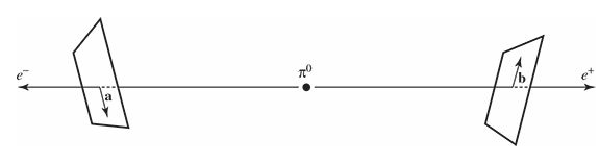
\includegraphics[width=0.75\textwidth]{figures/bell_scheme.eps}
    \caption{Belova postavka misaonog eksperimenta sa osama mjerenja koje mogu biti
        u proizvoljnim pravcima.}
    \label{fig:bell_exp_figure}
\end{figure}

Po\dj imo sada od pretpostavke da zaista postoji neka skrivena varijabla $\lambda$ koja omogućuje kompletniji opis stanja. Pošto se mjerenje može vršiti u bilo kojem pravcu, pretpostavimo da odabir pravca ne utiče na ishod mjerenja, već postoji neka funkcija koja je zavisna od skrivene varijable koja određuje ishod mjerenja.
Nazovimo funkciju koja određuje ishod mjerenja spina elektrona u pravcu $\vec{a}$, $A(\vec{a}, \lambda)$ i pozitorna u pravcu $\vec{b}$, $B(\vec{b}, \lambda)$.
Pošto ove funkcije utiču na ishod mjerenja, zaključujemo da su moguće njihove vrijednosti $\pm 1$.

Srednja vrijednost proizvoda pojedinačnih mjerenja je data sa

\begin{equation}
    P(\vec{a}, \vec{b}) = \int \rho (\lambda) A(\vec{a}, \lambda) B(\vec{b}, \lambda) d\lambda
\end{equation}
gdje smo sa $\rho (\lambda)$ označili gustinu vjerovatnoće skrivene varijable.
Ako posmatramo slučaj u kojem su detektori postavljeni u pravcima koji su međusobno paralelni, izmjerićemo uvijek suprotne spinove pa važi

\begin{equation}
    A(\vec{m}, \lambda) = - B(\vec{m}, \lambda).
\end{equation}
Srednja vrijednost proizvoda sada može da se napiše kao

\begin{equation}
    P(\vec{a}, \vec{b}) = - \int \rho (\lambda) A(\vec{a}, \lambda) A(\vec{b}, \lambda) d\lambda.
\end{equation}
Za bilo koji drugi jedinični vektor $\vec{c}$ važi takođe

\begin{equation}
    P(\vec{a}, \vec{c}) = - \int \rho (\lambda) A(\vec{a}, \lambda) A(\vec{c}, \lambda) d\lambda.
\end{equation}
Ako oduzmemo ove dvije jednačine dobijamo

\begin{equation}
    P(\vec{a}, \vec{b}) - P(\vec{a}, \vec{c})  = - \int \rho (\lambda) [A(\vec{a}, \lambda) A(\vec{b}, \lambda) - A(\vec{a}, \lambda) A(\vec{c}, \lambda) ] d\lambda.
\end{equation}
Zbog toga što je

\begin{equation}
    [A(\vec{b}, \lambda)]^2 = 1
\end{equation}
za proizvoljan vektor $\vec{b}$, drugi član u integrandu možemo pomnožiti sa takvom "jedinicom", pa dobijemo

\begin{equation}
    P(\vec{a}, \vec{b}) - P(\vec{a}, \vec{c})  = - \int \rho (\lambda) \left\{A(\vec{a}, \lambda) A(\vec{b}, \lambda) - A(\vec{a}, \lambda) A(\vec{c}, \lambda)[A(\vec{b}, \lambda)]^2 \right\}d\lambda.
\end{equation}
Jednostavnim izvlačenjem ispred zagrade dobijemo

\begin{equation}
    P(\vec{a}, \vec{b}) - P(\vec{a}, \vec{c})  = - \int \rho (\lambda) A(\vec{a}, \lambda) A(\vec{b}, \lambda) [1- A(\vec{c}, \lambda) A(\vec{b}, \lambda) ] d\lambda.
\end{equation}
Uzmimo sada apsolutnu vrijednost ovog izraza:

\begin{equation}
    \left|{P(\vec{a}, \vec{b}) - P(\vec{a}, \vec{c})}\right| =  \int \left| \rho (\lambda) A(\vec{a}, \lambda) A(\vec{b}, \lambda) [1- A(\vec{c}, \lambda) A(\vec{b}, \lambda)  ] \right| d\lambda.
\end{equation}
Pošto funkcije $A$ i $B$ uzimaju vrijednosti $\pm 1$ lako je vidjeti da je

\begin{equation}
    \left|A(\vec{a}, \lambda) A(\vec{b}, \lambda)\right| = 1.
\end{equation}

Analizirajmo sada član koji je preostao:

\begin{equation}
    \rho (\lambda)[1 - A(\vec{c}, \lambda) A(\vec{b}, \lambda) ].
\end{equation}
S obzirom da je $\rho(\lambda)$ gustina vjerovatnoće, kao takva funkcija mora biti ne-negativna tako da za taj član važi

\begin{equation}
    \rho(\lambda) \ge0 , \quad \forall \lambda.
\end{equation}
Proizvod $A(\vec{c}, \lambda) A(\vec{b}, \lambda)$ može imati vrijednosti $\pm 1$ tako da je

\begin{equation}
    1 - A(\vec{c}, \lambda) A(\vec{b}, \lambda) \ge 0 , \quad \forall \lambda.
\end{equation}
Dakle,

\begin{equation}
    \rho (\lambda)[1 - A(\vec{c}, \lambda) A(\vec{b}, \lambda) ] \ge 0, \quad \forall \lambda.
\end{equation}
Slijedi:


\begin{equation}
    \left|{P(\vec{a}, \vec{b}) - P(\vec{a}, \vec{c})}\right| \le  \int  \rho (\lambda)  [1- A(\vec{c}, \lambda) A(\vec{b}, \lambda)  ]  d\lambda = \underbrace{\int \rho(\lambda)d\lambda}_{1} + P(\vec{c}, \vec{b}).
\end{equation}
Konačno dobijemo Belovu nejednakost

\begin{equation}
    \left|{P(\vec{a}, \vec{b}) - P(\vec{a}, \vec{c})}\right| \le 1 +  P(\vec{c}, \vec{b}).
\end{equation}
Rezultat važi za bilo koju teoriju skrivenih varijabli, jer je $\rho(\lambda)$ proizvoljna funkcija raspodjele.

\section{Narušenje Belovih nejednakosti i implikacije}

Konstruišimo sada jednostavan primjer kojim možemo pokazati da dolazi do narušavanja Belovih nejednakosti. Na slici
su prikazana tri pravca u kojima možemo izvršiti mjerenje.

Želimo izračunati proizvod izmjerenih spinova po jednačini \eqref{eq:srednja_vrijednost_proizvoda}. Ako sa $\theta$ ozna\v cimo ugao me\dj u pravcima $\vec{a}$ i $\vec{b}$, onda se ova jedna\v cina mo\v ze napisati u obliku
\begin{equation}
    P(\vec{a},\vec{b}) = -cos\theta.
\end{equation}\\


% \begin{minipage}{0.6\textwidth}
% Your TikZ picture code here
\begin{tikzpicture}[scale=3, shift={(10,10)}]
    \def\arrowlength{1.5}

    % Arrow at 90 degrees
    \draw[->] (0,0) -- (\arrowlength,0) node[midway, below] {$\overrightarrow{b}$};

    % Arrow at 90 degrees
    \draw[->] (0,0) -- (0,\arrowlength) node[midway, left] {$\overrightarrow{a}$};

    \def\arrowlength{2}

    % Arrow at 45 degrees
    \draw[->] (0,0) -- (45:\arrowlength) node[midway, above, right] {$\overrightarrow{c}$};

    % draw arc
    \draw (0,0) -- (0.5,0) arc (0:45:0.5) -- cycle;
    \node at (0.3,0.15) {45\textdegree};
\end{tikzpicture}
\captionof{figure}{Detektori postavljeni sa relativnim uglovima od $45^\degree$ i $90^\degree$.}
\label{fig:detectors_with_chosen_angles}
% \end{minipage}

Ako izaberemo da ugao između pravaca $\vec{a}$ i $\vec{b}$ bude $90^\degree$, a uglovi ime\dj u pravaca $\vec{a}$ i $\vec{c}$, odnosno $\vec{b}$ i $\vec{c}$, po $45^\degree$ (slika: \ref{fig:detectors_with_chosen_angles}), Belova nejednakost glasi:
\begin{equation*}
    | cos(90^\degree) - cos(45^\degree)|\le 1 + cos(45^\degree).
\end{equation*}
Vidimo da ova nejednakost nije istinita, te zaključujemo da su Belove nejednakosti narušene.

